\section{Results}
\label{sec:psunc:results}

\subsection{$e^+e^-\to\text{jets}$}
\label{sec:psunc:results:ee}
Analysis: $91~\GeV$ and $500~\GeV$.

The C-parameter is defined as
\begin{equation}
  C = 3(\lambda_1\lambda_2 +\lambda_2\lambda_3 +\lambda_3\lambda_1)
  \label{eqn:cparam}
\end{equation}
where $\lambda_i$ are the eigenvalues of the linearised momentum tensor $\Theta^{\alpha\beta}$
\begin{equation}
  \Theta^{\alpha\beta} = \sum_i \frac{1}{|\vec{p}_i|} \sum_j \frac{\vec{p}^\alpha_j\vec{p}^\beta_j}{|\vec{p}_j|},\quad \alpha,\beta \in \{1,2,3\}
  \label{eqn:linearized_momentum_tensor}
\end{equation}
and satisfy
\begin{equation}
  \lambda_1\geq\lambda_2\geq\lambda_3,\quad\sum_i \lambda_i = 1
\end{equation}

Thrust:
\begin{equation}
  T = \max_{|\vec{n}_T|=1} \frac{\sum_i |\vec{p}_i\cdot \vec{n}_T|}{\sum_i |\vec{p}_i|}
  \label{eqn:thrust}
\end{equation}

\begin{figure}[h]
  \centering
  \begin{minipage}[t]{0.49\textwidth}
    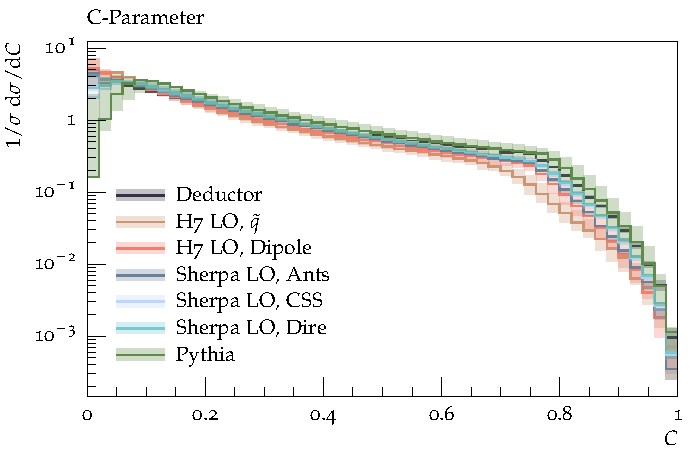
\includegraphics[width=1\textwidth]{plots/EE-91-MuShower/MC_EETOJETS/CParameter.pdf}
    \caption{Comparison of generator predictions for the C-parameter (\ref{eqn:cparam}) at $\sqrt{s}=91\GeV$ with uncertainty bands as described in \ref{}.}
    \label{fig:ee:cparam:91}
  \end{minipage}
  %
  \begin{minipage}[t]{0.49\textwidth}
    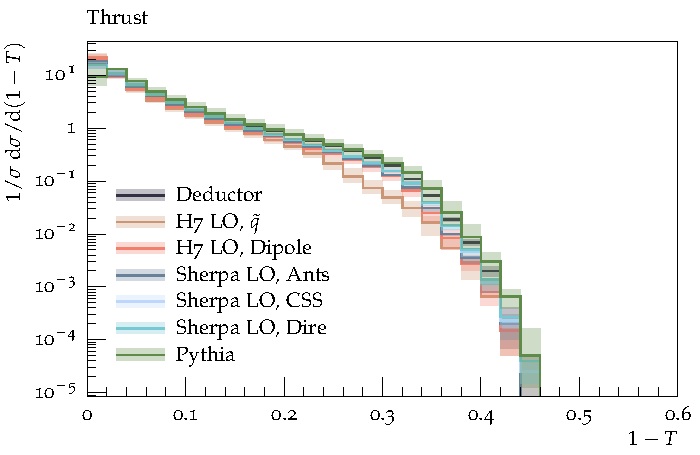
\includegraphics[width=1\textwidth]{plots/EE-91-MuShower/MC_EETOJETS/Thrust.pdf}
    \caption{Comparison of generator predictions for Thurst (\ref{eqn:thrust}) at $\sqrt{s}=91\GeV$ with uncertainty bands as described in \ref{}.}
	\label{fig:ee:thrust:91}
  \end{minipage}
\end{figure}

The Thrust  axis naturally separates an event into two hemispheres $H_U$ and $H_D$ that contain particles that are aligned, or anti-aligned with this axis. Specifically, these are defined by
\begin{equation}
  H_U = \{p_i ~|~ \vec{p}_i \cdot \vec{n}_T > 0\},\quad
  H_D = \{p_i ~|~ \vec{p}_i \cdot \vec{n}_T < 0\}.
\end{equation}
Jet mass squared in some region $R$ is given by: 
\begin{equation}
  \rho_R = \sum_{i\in R} \Big(\frac{p_i}{\sum_j p_j}\Big)^2
\end{equation}
Applying this to the hemispherical regions one can define a heavy-jet mass as:
\begin{equation}
  \rho_H = \max(\rho_U,\rho_D)
  \label{eqn:heavyjetmass}
\end{equation}



\begin{figure}[h]
  \centering
  \begin{subfigure}[t]{0.49\textwidth}
    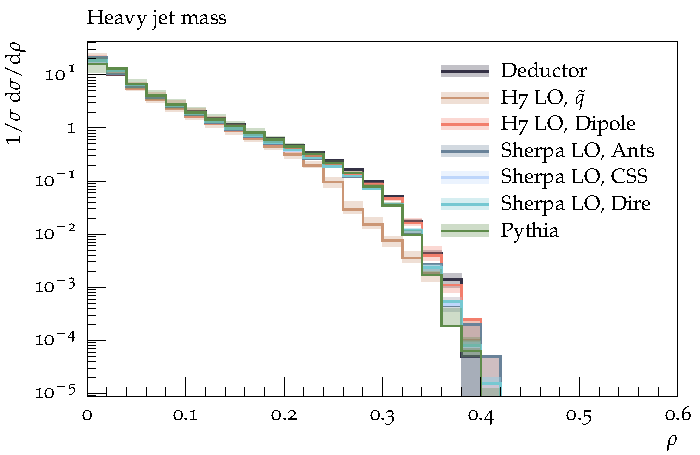
\includegraphics[width=\textwidth]{plots/EE-91-MuShower/MC_EETOJETS/HeavyJetMass.pdf}
    \caption{$\sqrt{s} = 91\GeV$}
    \label{fig:ee:heavyjetmass:91}
  \end{subfigure}
  %
  \begin{subfigure}[t]{0.49\textwidth}
    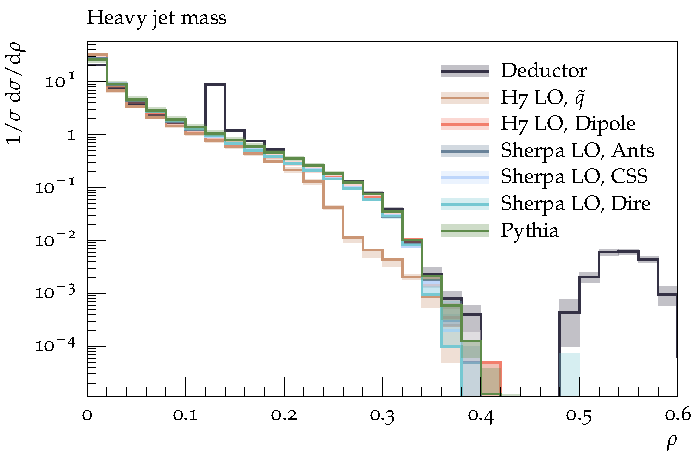
\includegraphics[width=\textwidth]{plots/EE-500-MuShower/MC_EETOJETS/HeavyJetMass.pdf}
    \caption{$\sqrt{s} = 500\GeV$}
    \label{fig:ee:heavyjetmass:500}
  \end{subfigure}
  \caption{Generator predictions for Heavy Jet mass (\ref{eqn:heavyjetmass}) at two different centre-of-mass energies.}
  \label{fig:ee:heavyjetmass}
\end{figure}

\begin{figure}[h]
  \centering
  \begin{subfigure}[t]{0.49\textwidth}
    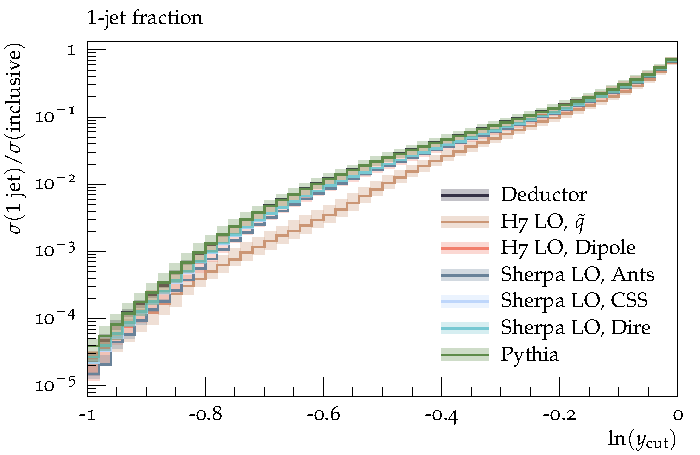
\includegraphics[width=1\textwidth]{plots/EE-91-MuShower/MC_EETOJETS/R1.pdf}
    \caption{1-jet fraction}
    % \label{fig:ee:cparam:91}
  \end{subfigure}
  %
  \begin{subfigure}[t]{0.49\textwidth}
    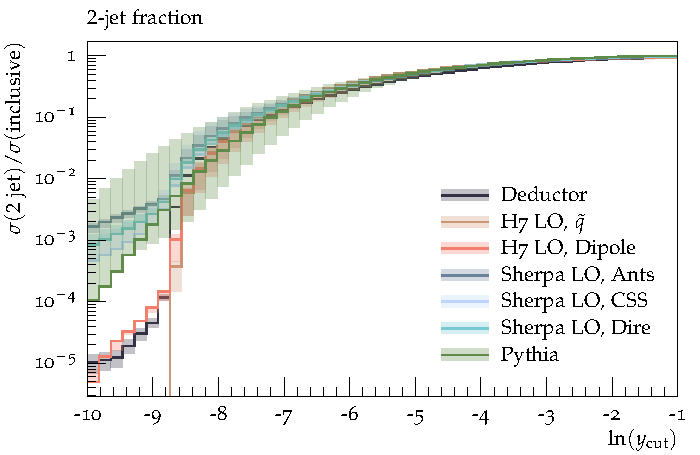
\includegraphics[width=1\textwidth]{plots/EE-91-MuShower/MC_EETOJETS/R2.pdf}
    \caption{2-jet fraction}
    % \label{fig:ee:thrust:91}
  \end{subfigure}
  \caption{Jet fractions at $\sqrt{s}=91\GeV$.}
\end{figure}

\begin{itemize}
  \item Deductor top-quarks in $500\GeV$ heavy jet mass. Peak at $\rho = (175/500)^2=0.1225$. New region with $0.49=(\frac{2*175}{500})^2 < \rho < \frac{(2*175 + 75)^2 - 75^2}{500^2}=0.7$
  \item Herwig deadzone in Thrust / R1
  \item Herwig behaviour at low $\ln(y_\textrm{cut})$ in $R2$ is the effect of the $1\GeV$ cutoff .
\end{itemize}

\subsection{$pp\to h$}
\label{sec:psunc:results:h}
Analysis: $13~\mathrm{TeV}$, $0.4$ Anti-$k_T$ jets with $p_{\perp,\mathrm{min}}=40\GeV$
\begin{figure}[h]
  \centering
  \begin{subfigure}[t]{0.49\textwidth}
    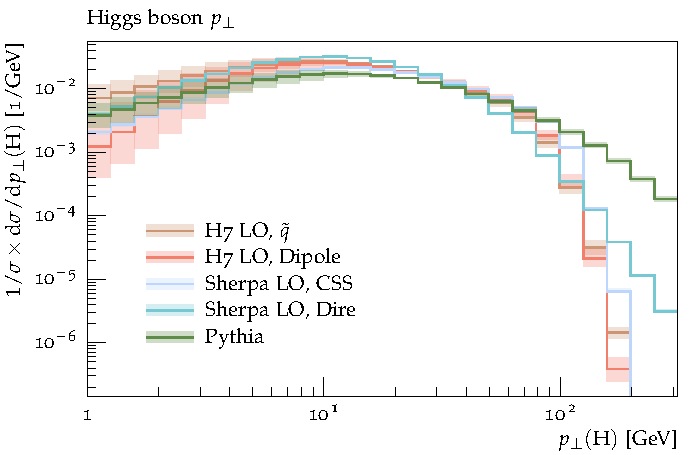
\includegraphics[width=\textwidth]{plots/H-125-MuShower/LH_H/X_pT.pdf}
    \caption{$H, pT$}
    \label{fig:h:pt_full}
  \end{subfigure}
%
  \begin{subfigure}[t]{0.49\textwidth}
    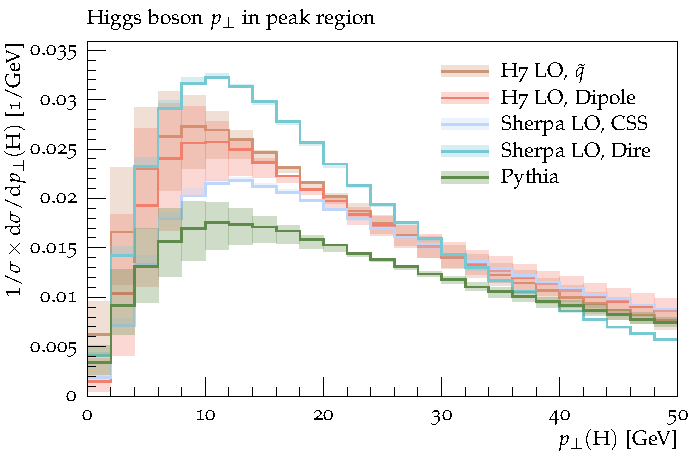
\includegraphics[width=\textwidth]{plots/H-125-MuShower/LH_H/X_pT_peak.pdf}
    \caption{$p_T$ in peak region}
    \label{fig:h:pt_peak}
  \end{subfigure}
  \caption{Generator comparison of the $H$ $p_\perp$ showing the overall behaviour \ref{fig:h:pt_full} as well as the behaviour in the peak region \ref{fig:h:pt_peak}}
  \label{fig:h:pt}
\end{figure}

\begin{figure}[h]
  \centering
  \begin{minipage}[t]{0.49\textwidth}
    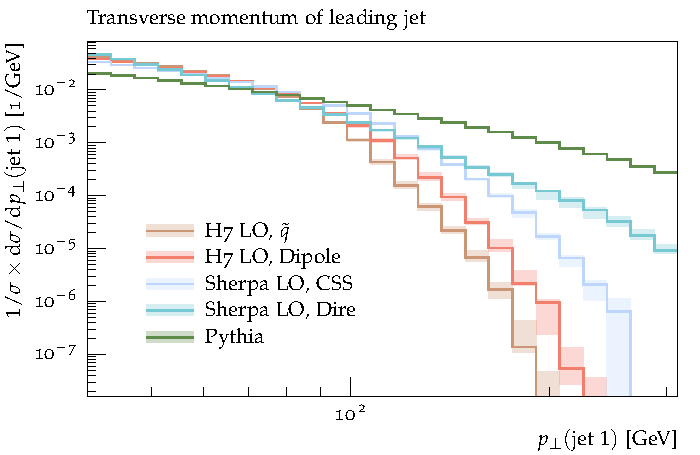
\includegraphics[width=1\textwidth]{plots/H-125-MuShower/LH_H/jet1_pT.pdf}
    \caption{$p_\perp$ of the leading jet (with $p_\perp > 40\GeV$)}
    \label{fig:h:jet1_pt}
  \end{minipage}
  %
  \begin{minipage}[t]{0.49\textwidth}
    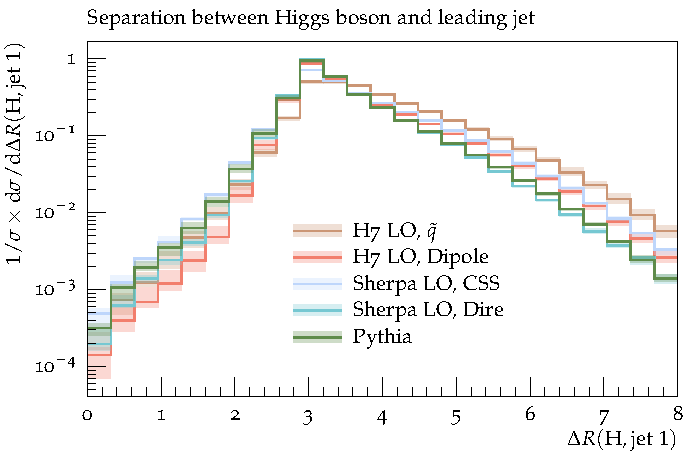
\includegraphics[width=1\textwidth]{plots/H-125-MuShower/LH_H/X_jet1_dR.pdf}
    \caption{Comparison for the lego-plot distance, $\Delta R = \sqrt{(\Delta\eta)^2 + (\Delta\phi)^2}$, between the Higgs and the leading jet.}
    \label{fig:h:deltaR}
  \end{minipage}
\end{figure}

\begin{figure}[h]
  \centering
  \begin{minipage}[t]{0.49\textwidth}
    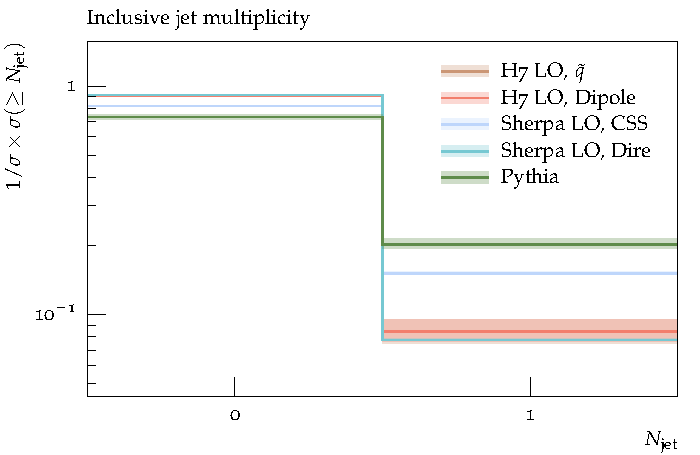
\includegraphics[width=1\textwidth]{plots/H-125-MuShower/LH_H/jet_multi_inclusive.pdf}
    \caption{Comparison for inclusive jet multiplicity.}
    \label{fig:h:jet_multi_inc}
  \end{minipage}
  %
  \begin{minipage}[t]{0.49\textwidth}
    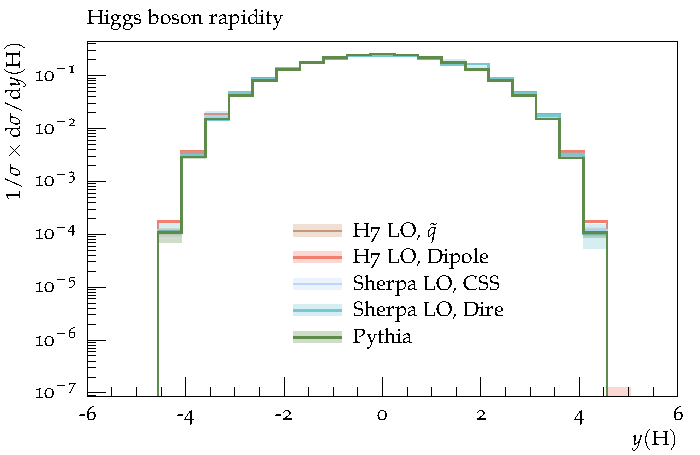
\includegraphics[width=1\textwidth]{plots/H-125-MuShower/LH_H/X_y.pdf}
    \caption{Higgs rapidity}
    \label{fig:h:y}
  \end{minipage}
\end{figure}


\subsection{$pp\to Z$}
\label{sec:psunc:results:dy}
Analysis: $13~\mathrm{TeV}$, $0.4$ Anti-$k_T$ jets with $p_{\perp,\mathrm{min}}=40\GeV$

\begin{figure}[h]
  \centering
    \begin{subfigure}[t]{0.49\textwidth}
    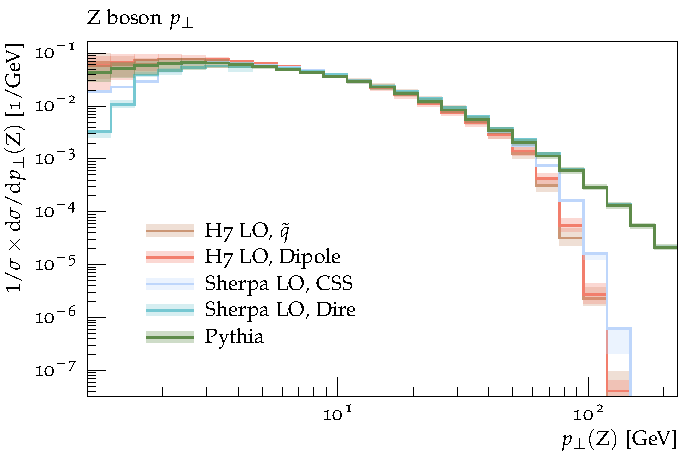
\includegraphics[width=\textwidth]{plots/Z-91-MuShower/LH_Z/X_pT.pdf}
    \caption{Entire region}
    \label{fig:z:pt_full}
  \end{subfigure}
%
  \begin{subfigure}[t]{0.49\textwidth}
    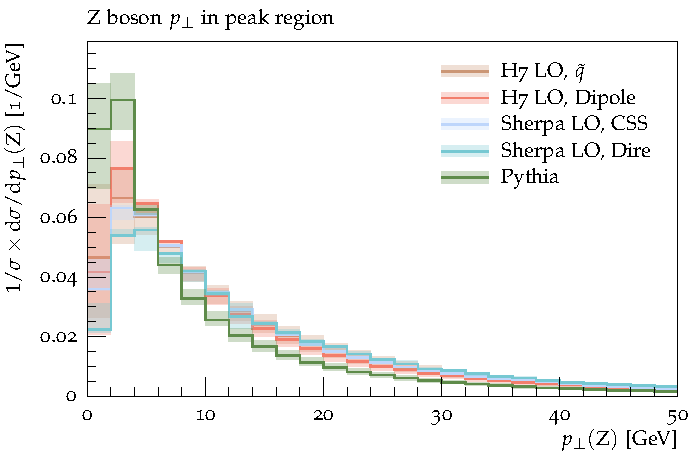
\includegraphics[width=\textwidth]{plots/Z-91-MuShower/LH_Z/X_pT_peak.pdf}
    \caption{Peak region}
    \label{fig:z:pt_peak}
  \end{subfigure}
  \caption{Generator comparison of the $Z$ $p_\perp$ showing the overall behaviour \ref{fig:z:pt_full} as well as the behaviour in the peak region \ref{fig:z:pt_peak}.}
  \label{fig:z:pt}
\end{figure}

\begin{figure}[h]
  \centering
  \begin{minipage}[t]{0.49\textwidth}
    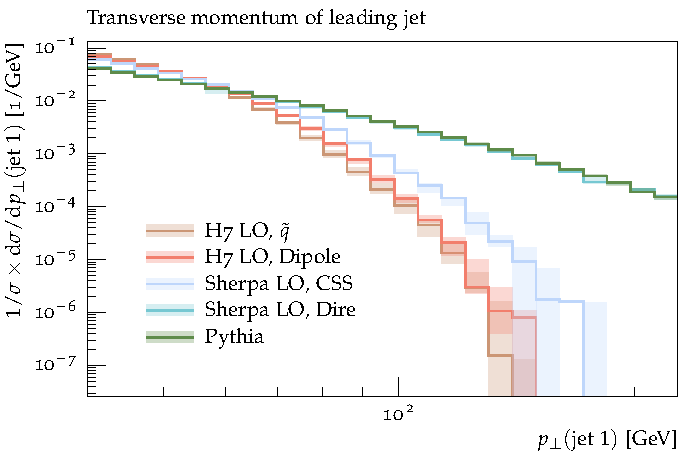
\includegraphics[width=1\textwidth]{plots/Z-91-MuShower/LH_Z/jet1_pT.pdf}
    \caption{$p_\perp$ of the leading jet (with $p_\perp > 40\GeV$)}
    \label{fig:z:jet1_pt}
  \end{minipage}
  %
  \begin{minipage}[t]{0.49\textwidth}
    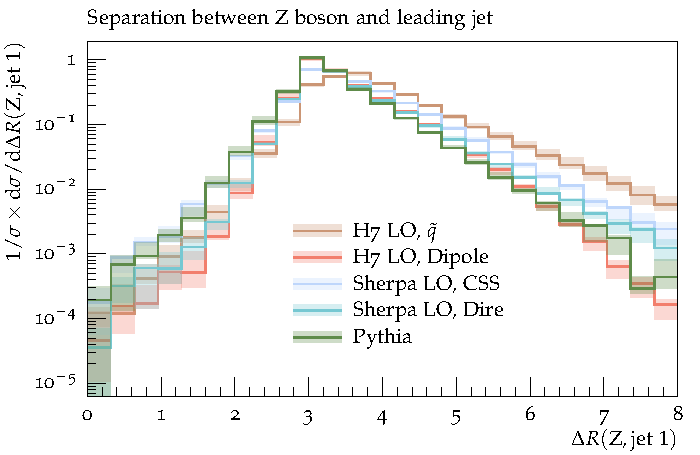
\includegraphics[width=1\textwidth]{plots/Z-91-MuShower/LH_Z/X_jet1_dR.pdf}
    \caption{Lego-plot distance, $\Delta R = \sqrt{(\Delta\eta)^2 + (\Delta\phi)^2}$, between the $Z$ and the leading jet.}
    \label{fig:z:deltaR}
  \end{minipage}
\end{figure}

\begin{figure}[h]
  \centering
  \begin{minipage}[t]{0.49\textwidth}
    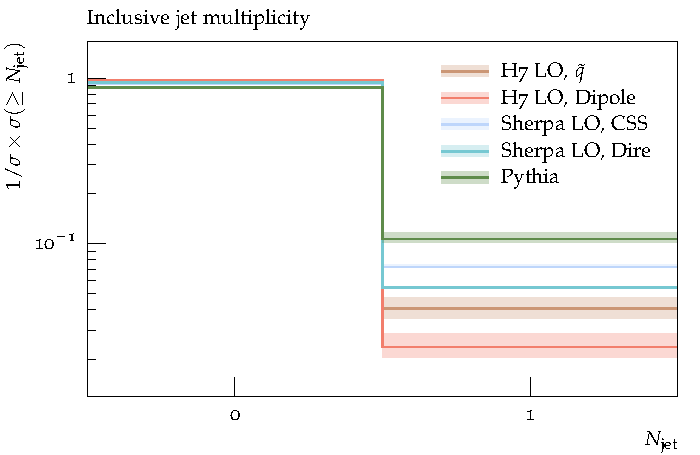
\includegraphics[width=1\textwidth]{plots/Z-91-MuShower/LH_Z/jet_multi_inclusive.pdf}
    \caption{Inclusive jet multiplicity}
    \label{fig:z:jet_multi_inc}
  \end{minipage}
  %
  \begin{minipage}[t]{0.49\textwidth}
    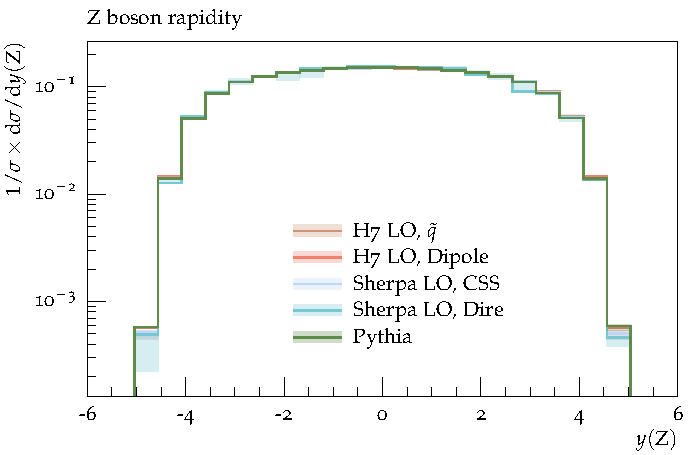
\includegraphics[width=1\textwidth]{plots/Z-91-MuShower/LH_Z/X_y.pdf}
    \caption{$Z$ rapidity}
    \label{fig:z:y}
  \end{minipage}
\end{figure}
